\documentclass[onecolumn]{aastex62}


\newcommand{\vdag}{(v)^\dagger}
\newcommand\aastex{AAS\TeX}
\newcommand\latex{La\TeX}
\usepackage{listings}
\usepackage{amsmath}
\usepackage{physics}
\usepackage{hyperref}
\usepackage{natbib}
\usepackage{wasysym}
\usepackage[T1]{fontenc}
\usepackage[english]{babel}
\usepackage[utf8]{inputenc}

\begin{document}

\title{\Large IN4200: Home exam I:\\Analysing web graphs.}



\author{Kandidatnr}



\section{Introduction} \label{sec:intro}
In this project we are going to implement a function for analysing data froma web graph file. The goal of this project is to outline the algorithms required for reading such a file and organising the data in both a $2$D table and on a compressed row storage format. Using both of these formats for storing the data we will show algorithms for computing the number of times each web page participates in a mutual linkage with another web page. The final goal of this project is to rank the webpages in a web graph with respect to the number of mutual linkages every web page participates in. The algorithms were tested with and without parallelization using openMP.
 
\section{Method} \label{sec:method}
\subsection{Format of a web graph file.}\label{sec:web}
When storing the data from the web graph file, one has to take into account how a web graph file stores its information. An example of a web graph file is shown below.
\begin{lstlisting}
# Directed graph (each unordered pair of nodes is saved once): 8-webpages.txt 
# Just an example
# Nodes: 8 Edges: 17
# FromNodeId    # ToNodeId
0   1
0   2
1   3
2   4
2   1
3   4
3   5
3   1
4   6
4   7
4   5
6   0
5   7
6   4
6   7
7   5
7   6
\end{lstlisting}
Nodes in this file represent the number of web pages that are included in the web graph. All nodes are given an Id with integer numbers ranging from zero to the amount of Nodes in the web graph. Edges represent the amount of times there is a link from one web page to another. The two columns FromNodeId and ToNodeId is the main data we are analysing. FromNodeId represents the Id of the web page with a link to the corresponding ToNodeId. From the first row in the example file we can see an example of this where Node 0 has a link to Node 1 and so forth.
\subsection{Storing the data from the file}
When storing the file in a $2$D table format one has to allocate a matrix with dimension Nodes$\times$Nodes. Along each row of the matrix we will store the amount of web pages that are linked to the given web page designated by the row, i.e, the first row designates the first web page and each element on that row designates designates all the other web pages in the web graph file. If a web page has a link to the web page belonging to the current row, the index of the the web page along the row will be given a value of $1$. If it does not link to the web page belonging to the row it will be given a value of zero. This continues for every row untill all web pages in the file has its own designated row thereby. To store the data in a $2D$ table format, we allocate a $2$D-array and set all elements to zero. When reading through the web graph file we set the web pages linking to the web page belonging to the designated row as \texttt{table2D[to][from] = 1}, where \texttt{to} is the current value on the ToNodeId column and \texttt{from} is the current value on the FromNodeId column. When doing this we have to make sure that we do not count if \texttt{from=to} as one web page can not link to itself giving the $2$D table zeroes on the diagonal.\\

When working with large web graph files, the 2D table format will store a lot of unneccesary information as zeroes. It is therefore convenient to introduce a much more, allthough a little bit more complicated, convenient format in terms of RAM usage. In this project we use the so called crompressed row storage format (CRS). In stead of storing all values as a matrix where alot of storage will be used to represent zeroes, we will now store our data in two arrays \texttt{row\_ptr} and \texttt{col\_idx}. The \texttt{col\_idx} array includes the index for each row where we have a value of one in the $2$D table. This array is of length $N_{links}$ which corresponds to the number of Edges in the web graph file. The \texttt{row\_ptr} array, starting at zero designating the first row, includes the index at which the \texttt{col\_idx} array changes row. This array is of length $N + 1$ where $N$ corresponds to the number of Nodes in the web graph file. With these two arrays we can store the same information as in the $2$D table but freeing up a lot of memory as we are only storing $N + 1 + N_{edges}$ integers instead of $N^2$ integers to account for all the zeroes in the 2D table. When creating these two arrays we start by reading through the web graph file and storing all the FromNodeId's and ToNodeId's in two arrays. At the same time  we update the \texttt{row\_ptr} array. Every time there is a linkage, it means that there should be one more element on each row belonging to the given web page being linked to.  This is is done by adding one to the array as \texttt{row\_ptr[to + 1]++}, where we index at \texttt{[to + 1]} since the first index zero is set to zero. When creating the \texttt{col\_idx} array one has to take into account that the data from the web graph file may be unsorted. (Forklar dette! Row ptr også ufullstendig forkalt).
\subsection{counting mutual links and top involvements}
When counting the mutual links, we refer to the number of times any two web pages has linked to the same web page. Number of involvements is the amount of times a given web page has taken part in a mutaul link. When counting the number of mutual linkages for the $2$D table one can find the amount of mutual by counting non-zero elements along the rows designating web pages linking to a certain node. If there are more than one element with a value of $1$ along each row there are webpages participating in a mutual linkage. To count the amount of mutual linkages we loop through all the rows and check if we find a non-zero value. If we find a non zero value we count all the remaining non-zero elements excluding the first element. The sum we then get is the amount of mutual links every web page along that row has contributed in. Then one can add the number of involvements for each of the web pages to a \texttt{num\_involvements} array indexed by the same index as their respective index in the table2D rows. The total number of mutual links will be a cumulative sum of all the rows as to not count web pages multiple times.\\

When extracting the same information from the CRS format, the same thought process is applied but the algorithm has to change with respect to the different storage format. The number web pages along each row is now determined by the \texttt{row\_ptr} array as \texttt{n\_pages = row\_ptr[i + 1] - row\_ptr[i]}. Once number of webpages is determined one can calculate the amount of linkages for each web page as \texttt{n\_pages - 1}. This value is then added to every web page with linkages inside the given \texttt{row\_ptr} interval. The total amount of mutual linkages will be a cumulative sum of defined by \texttt{n\_pages - 1} where we subtract $1$ from \texttt{n\_pages} for every iteration as long as \texttt{n\_pages>1}.
\subsection{ranking top involvements}
When counting the top involvements we start by looking at every value in the \texttt{top\_involvements} array. We then compare this value to every element in the \texttt{top\_n} array. If the web page we are looking at has more involvements than the one we are looking at in the \texttt{top\_n} array, we switch the value in the \texttt{top\_n} with the current value in the \texttt{top\_involvements} array and shuffle the remaining values in \texttt{top\_n} one step backwards. In this way we rank order the web pages by the number of times they have participated in a mutual link.\\

When parallelizing this algorithm we create an \texttt{top\_n} array with \texttt{n * nr\_threads} elements. we then divide the \texttt{top\_involvements} between the threads assigned to the problem. Each of these threads repeat the same algorithm as for the sequential approach, but we now store more values in our \texttt{top\_n} array which is now only ranked within the given interval worked worked on by a given thread. We then repeat the same algorithm on one thread, but now we loop through the \texttt{top\_n} and store the rank of the web pages we want in a shorter \texttt{top\_n\_shorter} array of length $n$. Allthough we have to do the algorithm twice on two separate arrays, the idea behind this is that we can shorten the time taken to loop through the \texttt{top\_involvements} by parallelizing it as this is the array with the most elements.
\section{Results}\label{sec:results}
These results were produced using an Intel core i7-6700 processor with 8 threads using the gcc compiler (gcc (Arch Linux 9.3.0-1) 9.3.0). All functions were compiled using the -O3 flag. When testing all the function on the web graph shown in section \ref{sec:web}, the 2D table turned out as 
\begin{equation*}
    \begin{pmatrix}
     0& 0 & 0& 0& 0& 0& 1& 0 \\
     1& 0 & 1& 1& 0& 0& 0& 0 \\
     1& 0 & 0& 0& 0& 0& 0& 0 \\
     0& 1 & 0& 0& 0& 0& 0& 0 \\
     0& 0 & 1& 1& 0& 0& 1& 0 \\
     0& 0 & 0& 1& 1& 0& 0& 1 \\
     0& 0 & 0& 0& 1& 0& 0& 1 \\
     0& 0 & 0& 0& 1& 1& 1& 0
    \end{pmatrix}.
\end{equation*}
For the same web graph the CRS format turned out as \texttt{col\_idx = [6 0 2 3 0 1 2 3 6 3 4 7 4 7 4 5 6]} and \texttt{row\_ptr  = [0 1 4 5 6 9 12 14 17]}. $13$ mutual links were counted with the number of involvements array turned out as \texttt{n\_involvements = [2 0 4 6 5 2 4 3 
]}. The web pages ranked in terms of involvements turned out as 
\begin{lstlisting}
    Web page nr 4 had 6 involvements
    Web page nr 5 had 5 involvements
    Web page nr 7 had 4 involvements
    Web page nr 3 had 4 involvements
    Web page nr 8 had 3 involvements
    Web page nr 6 had 2 involvements
    Web page nr 1 had 2 involvements
    Web page nr 2 had 0 involvements.
\end{lstlisting}
When timing the functions using a web graph containing $100$ nodes, our program clocked in at $0.165$ ms for storing the data as a $2$D array and $0.059$ ms for storing the data on a CRS format. The timing for the \texttt{count\_mutual\_links1} and \texttt{count\_mutual\_links2} functions using a varying number of threads is shown in figure \ref{fig:mutuallinks} using the same web graph with $100$ nodes. For the same web graph, figure \ref{fig:top_n} shows the time taken to rank the top $10$ web pages with a varying degrees of threads used in the paralellization. 
\begin{figure}
    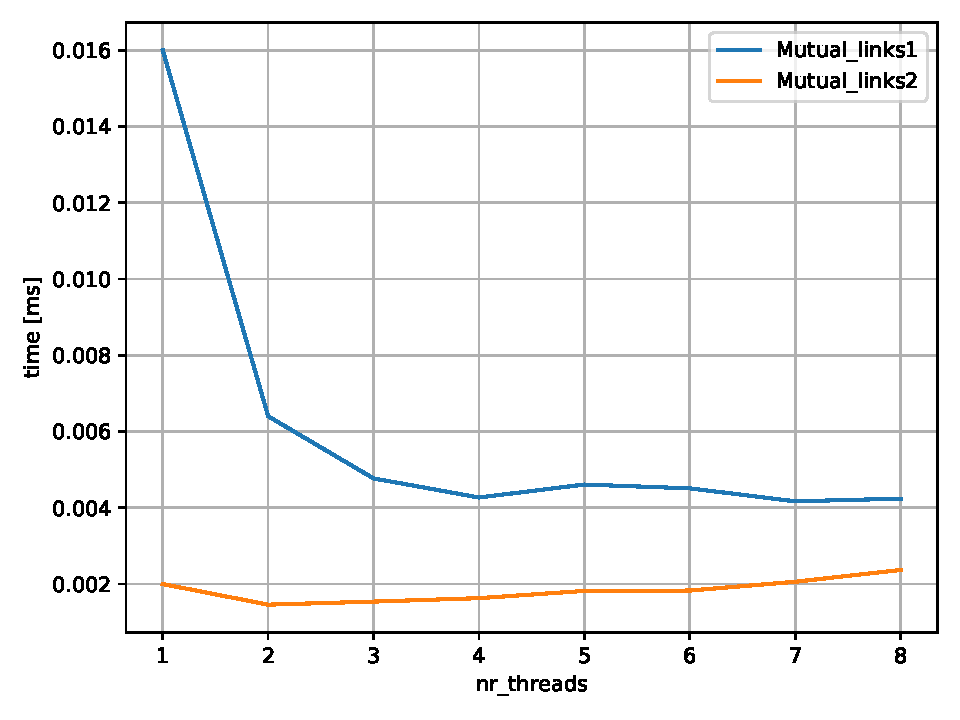
\includegraphics[scale=0.8]{figures/mutuallinks.pdf}
    \caption{Figure showing the time take for \texttt{count\_mutual\_links1} and \texttt{count\_mutual\_links2} functions on a webgraph with $100$ Nodes with a varying number of threads used.}
    \label{fig:mutuallinks}
\end{figure}
\begin{figure}
    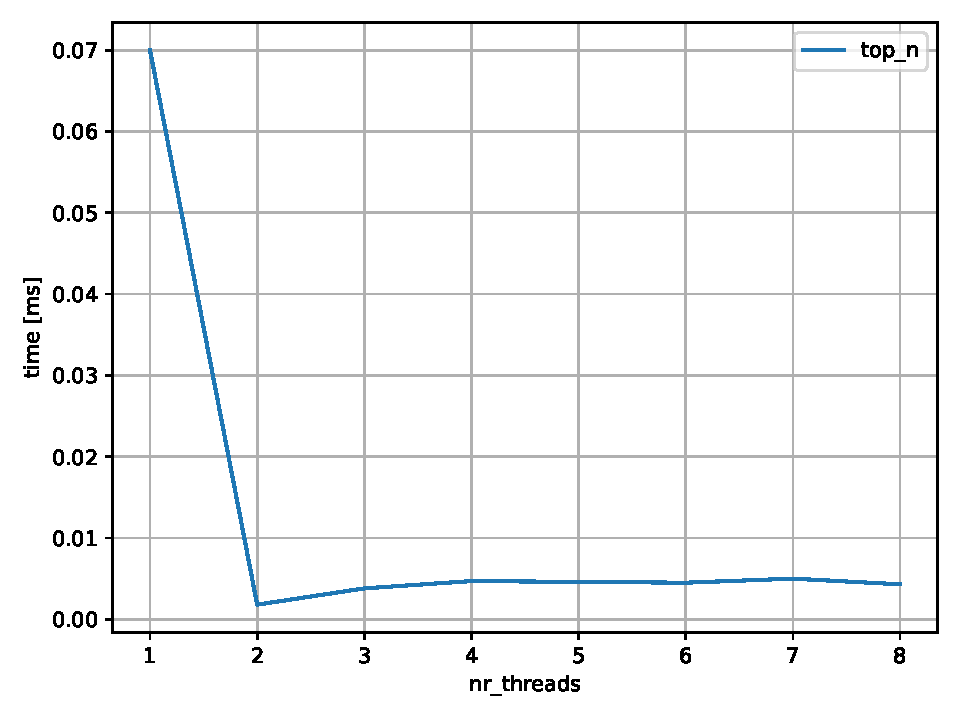
\includegraphics[scale=0.8]{figures/top_n.pdf}
    \caption{Figure showing the time take for the \texttt{top\_n} function on a webgraph with $100$ Nodes with a varying number of threads used. Note that here a slightly different algorithm had to be implemented for multiple threads.}
    \label{fig:top_n}
\end{figure}
\section{Discussion}
When determining the storage format, the CRS format is not only more memory efficient, but it also takes less time to execute. Allthough it is less intuitive than the 2D table format we did not find any other argument as to why one would not use the CRS format. Figure \ref{fig:mutuallinks} shows that the resulting algorithm from using the data stored on CRS format is also a lot more efficient than from reading the data from the $2$D table. Our results indicate that parallelizing has a lot more impact when reading the data from the $2$D table. from figure \ref{fig:mutuallinks} one can see that the $2$D table algorithm benefits the most when using $4$ threads before it flattens out. There is a minimal effect on parallelizing when reading the data from the CRS format. This can both be positive and negative. Not having to paralellize and still having better performance than the $2$D table method shows the benefits of the CRS format, but it can also indicate that our algorithm can be improved to better take advantage of parallelization. The timing when parallelizing the \texttt{top\_n} function shows that it benefits a lot from paralellization, but there aren't any benefits from using more than two threads. It is also worth noting that the file we tested was realatively short. Testing on a much larger file could make the sharing of the workload when looping over the \texttt{num\_involvements} much more effective.\\

We have implemented a set of functions for ranking the top web pages in terms of mutual linkages from a web graph file. Our results show that the CRS format is a superior storage format for sparse matrices. We show that the algorithms benefit from paralellization, but further insight in the effect of this could be gained by testing on larger files allthough this can be time consuming.

\bibliographystyle{aasjournal}
%\begin{thebibliography}{}
%\end{thebibliography}
\end{document}

% End of file `sample62.tex'.
